\chapter{Předzpracování série rentgenových snímků}

\subsection{Odstranění šumu průměrováním}
Digitální snímky pořízené pomocí běžných metod popsaných v literární rešerši obsahují šum, který vzniká v celém řetězci během pořizování snímku. Šum vzniká díky několika náhodným procesům:
\begin{itemize}
\item Počet fotonů, které opustí zdroj záření (Poissonovo rozdělení).
\item Počet fotonů, které projdou nedotčeně ozařovaným objektem. (binomické rozdělení)
\item Počet fotonů zachycených detektorem. (binomické rozdělení)
\item Počet světelných fotonů vygenerovaných ve scintilační vrstvě -- DR s nepřímým převodem. (binomické rozdělení)
\end{itemize}

Vzhledem k tomu, že výběr z fotonů generovaných procesem s Poissonovým rozdělení jsou opět fotony v Poissonově rozdělení, lze říci, že majoritní podíl šumu  digitálních snímcích má Poissonovo rozdělení. \cite{X-ray-imaging-noise-and-SNR} Jednou z metod pomocí které lze tento šum odstranit je průměrování.

\paragraph{Průměrování}
je jednoduchou metodou pro odstranění šumu, která je velmi citlivá na odchylky vzniklé změnou pozice snímaného objektu v obraze. Tato metoda lze popsat pomocí následující rovnice:

\begin{equation}
\label{eq:average}
I_{filtered} \left( x,y \right ) = \frac{1}{N} \sum_{i = 0}^{N - 1}I_{i}\left( x,y \right ),
\end{equation}
kde $x$ a $y$ jsou index pixelů, $N$ počet snímků v množině snímků a $I_{i}$ i-tý snímek z množiny snímků.

Citlivost této metody na odchylky vzniklé změnou pozice objektu v obraze lze řešit pomocí metod založených na \zkratka{zk:AAR}. Tyto metody spočívají v předzpracování množiny snímků pomocí metod registrace obrazových dat a následném průměrování podle rovnice \ref{eq:average}.

\subsubsection{Průmerování po registraci (AAR)}
Hlavní problém, který tato metoda řeší je hledání stejných klíčových bodů mezi páry $\left\{ I_{i}, I_{j} \right\}$ pro $j = \left \{0, 1, ..., N - 1 \right \} - \left \{i \right \}$, kde $I$ je množina všech snímků, $i$ je index základního snímku vůči kterému jsou hledány klíčové body ve snímcích $I_{j}$ a $N$ je celkový počet snímků v množině $I$. Jinými slovy tato metoda spočívá v nalezení stejných klíčových bodů mezi základním snímkem například $S_{0}$ a ostatními snímky $S_{j}$ z množiny všech snímků $I$. K hledání stejných klíčových bodů mezi páry tato metoda využívá deskriptorů. Po nalezení stejných klíčových bodů je nutné na základě těchto bodů transformovat snímek $S_j$ do souřadnicové soustavy základního snímku. Po transformaci všech snímků do souřadnicové soustavy základního snímku je možné všechny snímky zprůměrovat podle rovnice \eqref{eq:average} a tím odstranit šum. Tento postup popisuje \cref{fig:AAR-flowchart}

\begin{figure}[htb]
\centering
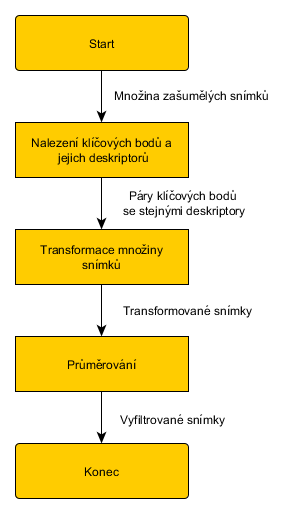
\includegraphics[width=7cm]{AAR-flowchart}
\caption{Vývojový diagram metody \zk{zk:AAR}.}
\label{fig:AAR-flowchart}
\end{figure}

\paragraph{ORB (Oriented FAST and rotated BRIEF)}
je metoda pro hledání klíčových bodů a jejich deskriptorů založena na metodách FAST (detektor klíčových bodů) a BRIEF (binární deskriptor). Tato metoda byla na vržena jako méně výpočetně náročná alternativa k metodám \zkratka{zk:SIFT} a \zkratka{zk:SURF}. Mimo nižší výpočetní náročnost dosahuje metoda \zk{zk:ORB} lepších výsledků vzhledem k natočení zkoumaného snímku (\cref{fig:orb-comparsion}). Další výhodou \zk{zk:ORB} oproti metodám \zk{zk:SURF} a \zk{zk:SIFT} je, že je vydána pod otevřenou licencí BSD, čili je oproti \zk{zk:SURF} a \zk{zk:SIFT}, které jsou patentovány zdarma. \cite{orb}
\begin{figure}[htb]
\centering
\includegraphics[width=\textwidth]{orb-comparsion}
\caption{Porovnání úspěšnosti hledání klíčových bodů a jejich deskriptorů pro různé metody v závislosti na rotaci snímku. \cite{orb}}
\label{fig:orb-comparsion}
\end{figure}

\paragraph{BRIEF} je metoda pro určování binárních deskriptorů \zk{zk:ORB}, která pracuje na principu testování intenzity náhodně vybraných bodů v konkrétní části snímku, která má velikost $S \times S$. Tento test lze definovat jako:

\begin{equation}
\label{eq:BRIEF-test}
\tau \left (p; x,y \right ):= \left\{\begin{matrix}
1 & pro \quad p\left( x\right ) < p \left(y \right )\\ 
0 & pro \quad p\left( x\right ) \geq  p \left(y \right )\\ 
\end{matrix}\right.,
\end{equation}
kde $\tau$ je výsledek testu, $p\left(x\right)$ a $p\left(y\right)$ jsou intenzity pixelů na indexech $x$ a $y$ a $p$ je zkoumaná část snímku na kterou  je test prováděn. Zkoumaná část snímku $p$ by měla být vyhlazena vyhlazovacím filtrem. Výběrem náhodných indexů $x$ a $y$ z části snímku $p$ je vytvořena sada binárních testů, kterou lze definovat jako:

\begin{equation}
\label{eq:BRIEF-test-set}
f_{n_{d}} \left(p \right ) = \sum_{1\leq i\leq n_{d}} 2^{i-1} \tau \left(p; x_i, y_i \right ).
\end{equation}
Z rovnice \ref{eq:BRIEF-test-set} plyne, že deskriptor $f_{n_d}$ se bude skládat z $2^{n_d}$ výsledků testů. \cite{brief} V případě implementace pro \zk{zk:ORB} je velikost deskriptoru $n = 256$. Jak již bylo zmíněno před aplikací metody BRIEF je nutné zkoumanou část snímku nejprve vyhladit. V případě \zk{zk:ORB} je vyhlazení prováděno pomocí integračního vyhlazovacího operátoru o velikosti okna $5 \times 5$ na zkoumanou část snímku a velikosti $31 \times 31$ pixelů. Problémem metody BRIEF je, si nedokáže dobře poradit s natočenými snímky. Proto je BRIEF v rámci \zk{zk:ORB} rozšířen o natočení podle klíčových bodů. \cite{orb}

\paragraph{FAST} je metodou pro detekci klíčových bodů ve snímku. Tato metoda je založena na detekci hran pomocí kruhového okolí. Algoritmus nejprve vybere pixel $\rho$  o intenzitě $I_\rho$ u kterého má být určeno, zda je hranou, či ne. Následně je zvolen vhodný práh $t$ a kruhové okolí pixelu $\rho$ o velikosti 16 pixelů. Pixel je následně považován za hranu v případě, že se po obvodu kruhového okolí nachází souvislá množina pixelů, jejichž intenzita je vyšší nebo nižší než intenzita $I_\rho$. 

Mimo postupu, jenž je popsaný výše existuje varianta, která se snaží urychlit  celkový proces hledání hran. Tato metoda spočívá ve zkoumání pouze pixelu číslo 1, 9, 5 a 13. Jestliže jsou pixely 1 a 9 vyhodnoceny jako tmavší nebo světlejší než $I_\rho + t$, pak jsou stejným způsobem otestovány i pixely 5 a 13. Pixel je považován za hranu v případě, že alespoň 3 z množiny pixelů jsou světlejší nebo tmavší než $I_\rho + t$. \cite{rosten_2008_faster}.

V případě implementace v \zk{zk:ORB} je využit FAST s kruhovým okolím 9. Vzhledem k tomu, že FAST neurčuje orientaci, byla tato metoda v rámci \zk{zk:ORB} rozšířena o určení orientace pomocí centroidu. \cite{orb}

\begin{figure}[htb]
\centering
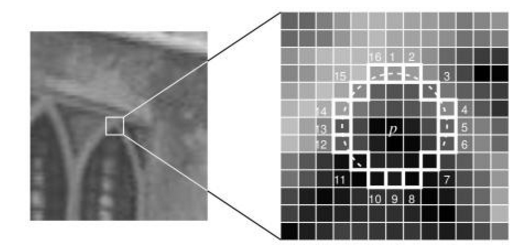
\includegraphics{fast}
\caption{Princip výběru okolí a způsob indexování pixelů metody FAST. \cite{rosten_2008_faster}}
\label{fig:fast}
\end{figure}

\paragraph{RANSAC (Random sample consensus)} je metoda sloužící k nalezení modelu, který definuje vztah mezi dvěma lineárně závislými množinami. Tato metoda pracuje s předpokladem, že k definování lineárního modelu stačí pouze dva body (na rozdíl od metody nejmenších čtverců, která předpokládá, že velké množství dat dokáže eliminovat odchylky). Algoritmus této metody lze popsat pomocí následujících bodů \cite[str.~462]{Image-Processing-Analysis-and-Machine-Vision}:
\begin{enumerate}
\item Uvažujeme množinu bodů $X = \left\{x_1, x_2, ..., x_n \right\}$ u které předpokládáme, že odpovídá modelu, který je určen alespoň $m$ body z množiny. Například pro přímku $m = 2$.
\item Nastavíme čítač iterací $k$ na hodnotu 1.
\item Náhodně vybereme $m$ bodů z množiny a vypočítáme model (například pomocí metody nejmenších čtverců).
\item S odchylkou $\eta$ určíme kolik bodů z množiny odpovídá modelu. Pokud počet překročí práh $t$, model se přepočítá z bodů, které odpovídají modelu.
\item Zvýšíme čítač iterací o 1 a zkontrolujeme zda $k < K$, kde $K$ je maximální počet iterací. Pokud $k < K$ pokračujeme bodem 3, jinak ukončíme algoritmus a jako model zvolíme ten, kterému odpovídalo nejvíce bodů z modelu.
\end{enumerate}
Takto získaný model lze poté využít jako model pro transformaci souřadnicové soustavy jendoho snímku do souřadnicové soustavy druhého snímku. Jako body, na základě kterých je model vytvářen lze použít klíčové body získané pomocí ORB. 

\subsubsection{Implementace}
Na základě metod popsaných výše lze implementovat algoritmus pro odstranění šumu průměrováním. Navržený algoritmus (obrázek \ref{fig:AAR-flowchart-implementation}) upřesňuje postup z obrázku \ref{fig:AAR-flowchart} o konkrétní operace.

\begin{figure}[!htb]
\centering
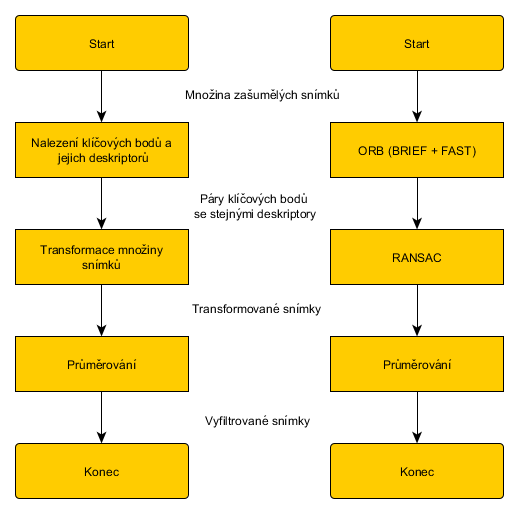
\includegraphics[width=12cm]{AAR-flowchart-implementation}
\caption{Vývojový diagram AAR s konkrétně zvolenými metodami pro jednotlivé operace. \zk{zk:AAR}.}
\label{fig:AAR-flowchart-implementation}
\end{figure}

Celý postup je implementován pomocí jazyka Python v prostředí Jupyter notebook. V implementaci je využito knihovny scikit-image, která poskytuje nástroje pro práci s obrázky včetně implementovaných metod ORB a RANSAC. Pro zobrazení výsledků je použit balíček pro zobrazování grafů matplotlib a pro matematické operace (především pro práci s maticemi) je využíváno balíčku numpy.

\subsubsection{Testovací data}
Za účelem ověření implementovaného postupu byla nasnímány a předzpracovány testovací snímky. Jako zdroj záření byla zvolena rentgenka Spellman XRB011 \cite{spellman-xrb011} s maximálním napětím v rozmezí od \SI{35}{\kV} do \SI{80}{\kV} a žhavícím proudem od \SI{0}{\micro\ampere} do \SI{700}{\micro\ampere}. Snímání záření poté obstarává flat-panel s CMOS snímači Shad-o-Box 1548 HS \cite{SB1548HS} od společnosti Teledyne Dalsa. Rozlišení detektoru je $1032 \times 1548$ a velikost snímací plochy je $\SI{10.2}{\cm} \times \SI{15.3}{\cm}$. Maximální snímkovací frekvence 30 snímku za vteřinu.

Pomocí této sestavy bylo nasnímáno 20 stejných snímků v časovém rozmezí \SI{20}{\second} mezi jednotlivými snímky. Snímky byly nasnímány s \SI{60}{\kV} a \SI{250}{\micro\ampere} na rentgence při době expozice \SI{30}{\ms}. Jeden ze série nasnímaných snímků lze vidět na obrázku \ref{fig:averaging-dataset-sample} (A). Ve snímku je patrný již zmiňovaný šum s Poissonovým náhodným rozdělením. 

\begin{figure}[htb]
\centering
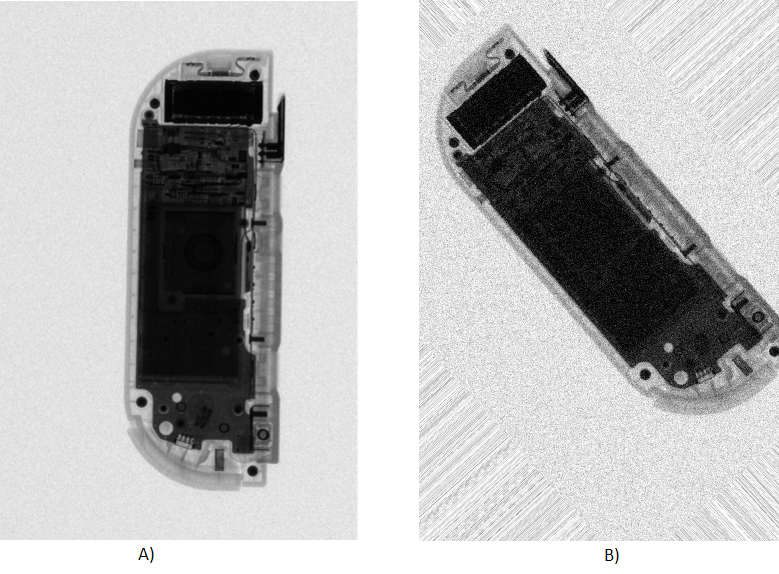
\includegraphics[width=\textwidth]{averaging-dataset-sample}
\caption{Jeden snímek JoyConu konzole Nintendo Switch ze série testovacích snímků (A) a jeho podoba po aplikaci umělého šumu (B).}
\label{fig:averaging-dataset-sample}
\end{figure}

\paragraph{Předzpracování série testovacích snímků} 
bylo provedeno za účelem zhodnocení robustnosti implementované metody. Předzpracování bylo zaměřeno především na aplikaci umělého šumu na testovací data. Byly vytvořeny dvě testovací množiny s různými úrovněmi šumu:
\begin{enumerate}
\item Vyšší úroveň šumu
\begin{itemize}
\item Posunutí snímku v osách $x$ a $y$ o náhodný počet pixelů v intervalu $\left \langle -200,200 \right \rangle$.
\item Rotace snímku podle jeho středu o náhodnou velikost úhlu v intervalu $\left \langle -190,190 \right \rangle$ stupňů.
\item Aplikace náhodného šumu v Gaussově rozložení s variancí $\sigma^2 = 0.01$.
\end{itemize}
\item Nižší úroveň šumu
\begin{itemize}
\item Posunutí snímku v osách $x$ a $y$ o náhodný počet pixelů v intervalu $\left \langle -20,20 \right \rangle$.
\item Rotace snímku podle jeho středu o náhodnou velikost úhlu v intervalu $\left \langle -20,20 \right \rangle$ stupňů.
\item Aplikace náhodného šumu v Gaussově rozložení s variancí $\sigma^2 = 0.01$.
\end{itemize}
\end{enumerate}

Předzpracovaný snímek po aplikaci vyšší úrovně šumu 1) ukazuje obrázek \ref{fig:averaging-dataset-sample} (B). Díky náhodnému posunu a rotaci snímku ve snímku vznikají prázdné pixely. Hodnota těchto pixelů je nastavena na hodnotu hran snímku. Tento jev lze také sledovat na obrázku \ref{fig:averaging-dataset-sample} (B) jako pruhované oblasti v okolí originálního snímku.

\subsubsection{Výsledky aplikace metod pro odstranění šumu}
Na uměle zašumělá data byl aplikován algoritmus obyčejného průměrován, který je porovnán s výsledky algoritmu AAR. Algoritmus byl aplikován na snímky s oběmi úrovněmi šumu, které byly specifikovány výše. Výsledky aplikace algoritmů pro nízký šum ukazuje obrázek \ref{fig:averaging-low-noise} a pro vysoký šum obrázek \ref{fig:averaging-high-noise}.

V detailech obrázku \ref{fig:averaging-low-noise} (C a D) je zřejmý vliv obrazové registrace před průměrováním, kde díky transformaci snímků do stejné  souřadnicové soustavy pomocí ORB a RANSAC nejsou v detailu D viditelné artefakty způsobené odchylkami pozic testovacích snímků. Tyto artefakty jsou naopak viditelné na detailu C, u kterého transformace provedena nebyla.

Výsledky na obrázku \ref{fig:averaging-high-noise} dokazují robustnost metody AAR. Ve snímku A se nachází průměr všech snímků na který byla aplikována vysoká úroveň šumu. Ze snímku je patrný veliký rozsah natočení a posunutí v osách $x$ a $y$ při aplikaci vysoké úrovně šumu. Druhý snímek B obrázku \ref{fig:averaging-high-noise} ukazuje robustnost implementované metody AAR. Ve snímku jsou patrné artefakty v okolí snímaného předmětu. Tyto artefakty jsou způsobeny nahrazováním prázdných pixelů při aplikaci šumu hodnotami hran snímku. V reálných podmínkách, kdy není šum aplikován uměle by tyto artefakty byly potlačeny.

Implementací a aplikováním metody AAR se podařilo navrhnout robustní metodu pro odstranění náhodného šumu v rentgenových snímcích. Tato metoda je odolná proti šumu, který může být způsoben náhodným posunem a rotací snímaného objektu v pořízeném snímku. Díky této vlastnosti lze implementovanou metodu využít například pro odstranění šumu při rentgenování pohybujícího se objektu  .

\begin{figure}[htb]
\centering
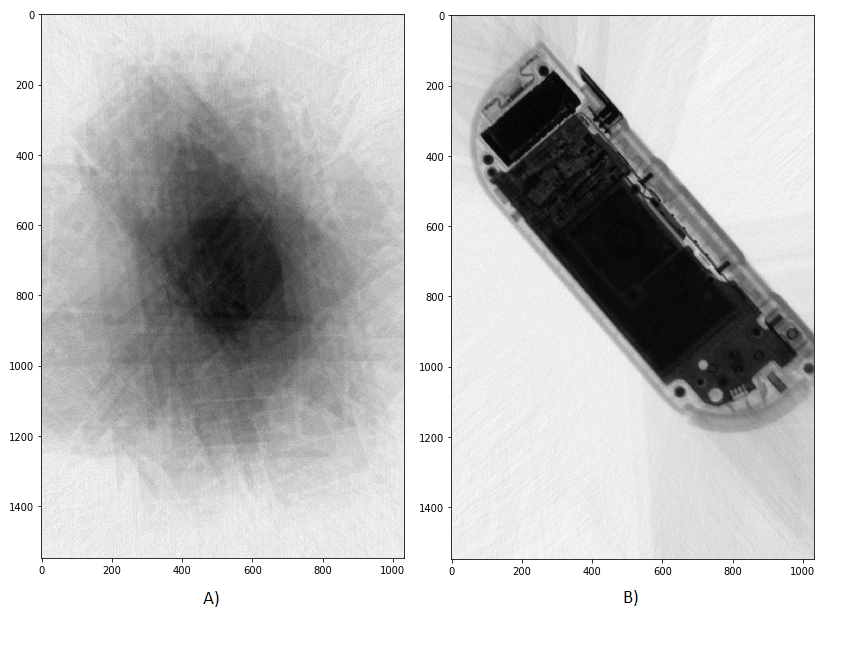
\includegraphics[width=\textwidth]{averaging-highnoise}
\caption{Jeden snímek JoyConu konzole Nintendo Switch ze série testovacích snímků (A) a jeho podoba po aplikaci umělého šumu (B).}
\label{fig:averaging-high-noise}
\end{figure}

\begin{figure}[htb]
\centering
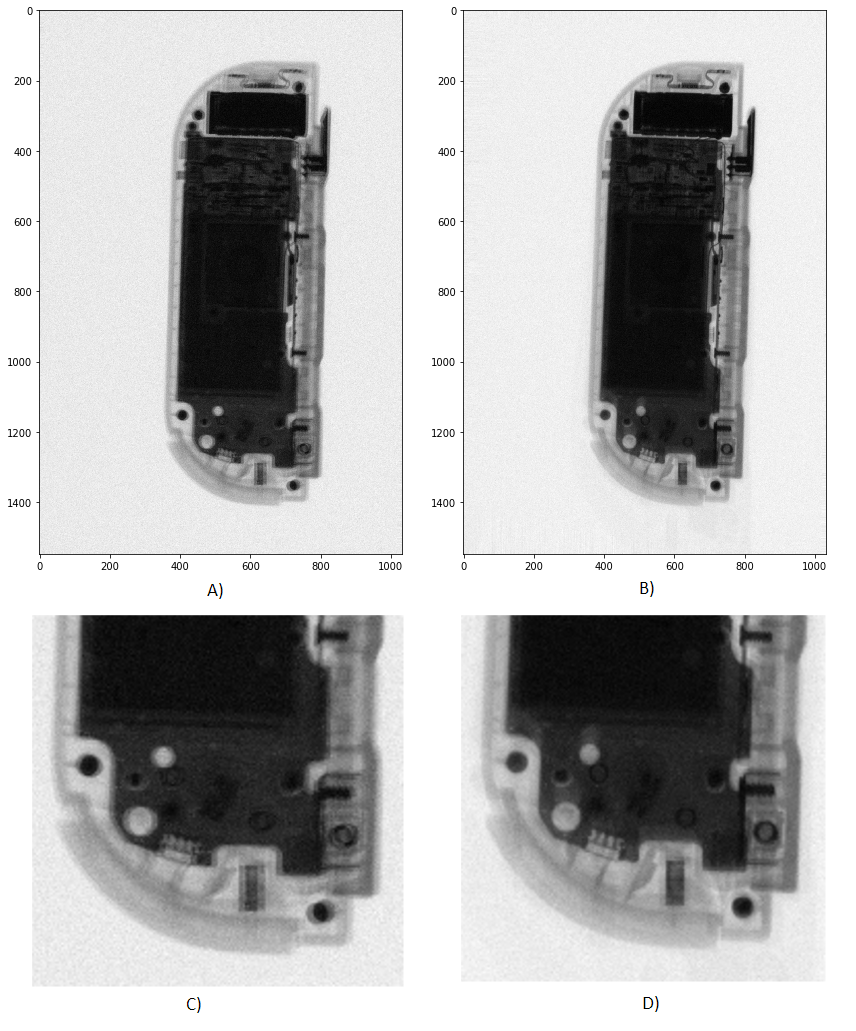
\includegraphics[width=\textwidth]{averaging-lownoise}
\caption{Jeden snímek JoyConu konzole Nintendo Switch ze série testovacích snímků (A) a jeho podoba po aplikaci umělého šumu (B).}
\label{fig:averaging-low-noise}
\end{figure}
\clearpage

\subsection{Zvýšení dynamického rozsahu metodou HDR (High Dynamic Range)}
Uvážíme-li situaci, kdy snímáme scénu a jako výsledek snímání obdržíme dvourozměrné pole změřených hodnot intenzity záření, tak nelze říct, že naměřené hodnoty intenzity přímo odpovídají záření ve scéně. Jinými slovy je nepravděpodobné, že pokud jedna hodnota intenzity je dvojnásobná oproti druhé, tak dopadající záření odpovídající druhé hodnotě je dvojnásobné. Tuto situaci lze sledovat především u filmových systémů, v případě systémů DR s přímým a nepřímým převodem bývá tento jev potlačen -- odezva detektoru je částečně lineární.

Tato nelinearita je dle \cite{Debevec} nazývána nelineární mapování. Vznik nelinearity při převodu záření na digitální snímek závisí především na konstrukci detektoru (scintilační vrstva, typ receptoru apod.). \cite{Debevec}
Odezva detektoru na expozici $X$ bývá označována jako charakteristická křivka detektoru.

Jak u filmových, tak u DR systémů se můžeme setkat s nelinearitou, která je způsobena saturací detektorů, která omezuje dynamický rozsah detektorů. V případě, že jsou ve snímané scéně zájmové oblasti s vysokou a nízkou intenzitou záření, není díky nízkému dynamickému rozsahu detektoru možné pozorovat detaily obou oblastí -- jedna z oblastí je vždy změnou doby expozice, urychlovacího napětí nebo žhavícího proudu posunuta mezi saturační body na charakteristické křivce a druhá oblast do oblasti saturace. Pokud chceme pokrýt celý dynamický rozsah musíme pořídit sérii snímků s různými dobami expozice, hodnotami proudu nebo napětí. Metody HDR se zabývají sloučením takto pořízených snímků v jeden snímek schopný zobrazit scénu s vysokým dynamickým rozsahem. 
Tyto metody pracuji na principu vytvoření mapy popisující intenzitu záření ve scéně, které je pak využita pro škálování hodnot intenzit digitálního snímku. 
Jednou z těchto metod popsané v \cite{Debevec} je metoda navržena Paulem E. Debevecem.

\subsubsection{Debevec HDR}
Tato Metoda pro získání snímku s vysokým dynamickým rozsahem sloučením série snímků získaných s rozdílnými expozičními dobami se skládá ze dvou částí:

\begin{itemize}
\item estimace charakteristické křivky / funkce odezvy detektoru a
\item sloučení série snímků -- vytvoření HDR snímku.
\end{itemize}
\paragraph{Estimace odezvy detektoru} je založena na principu reciprocity. Tento princip říká, že je-li expozice $E$ definována jako:
\begin{equation}
\label{eq:debevec_reciprocity}
X = E \Delta t , 
\end{equation}
kde $E$ ozáření detektoru a $\Delta t$ doba expozice, tak při dvojnásobném snížení $E$ a dvojnásobném zvýšení $\Delta t$ se nezmění změřená hodnota intenzity. Charakteristická křivku převodu expozice $X$ na digitální snímek $Z$ lze vyjádřit pomocí funkce $f$ jako:
\begin{equation}
\label{eq:debevec_char}
Z=f\left (X \right ) \Leftrightarrow X = f^{-1}\left ( Z\right ). 
\end{equation}
Vzhledem k tomu, že $f$ je monotónní, lze expozici $X$ získat pomocí invertované funkce $f^{-1}(Z)$, jak ukazuje rovnice \ref{eq:debevec_char}. Rovnici \ref{eq:debevec_char} po dosazení za $X$ podle rovnice \ref{eq:debevec_char} lze aplikovat na sérii digitálních snímků jako:
\begin{equation}
\label{eq:debevec_char_ap}
Z_{ij}=f\left (E_i\Delta t_j \right ) \Leftrightarrow f^{-1}\left ( Z_{ij}\right ) = E_i \Delta t_j\quad,
\end{equation}
kde i je index pixelu ve snímku a j index snímku / doby expozice. Po aplikování přirozeného logaritmu na obě strany rovnice a zavedení substituce  $g(Z_{ij} = \ln\left( f^{_1} \right))$ je výsledná rovnice:
\begin{equation}
\label{eq:debevec_char_ap_fin}
g \left( Z_{ij} \right) = \ln \left( E_i \right)  + \ln \left( \Delta t_j \right),
\end{equation}
kde $Z_{ij}$ a $\Delta t_j$ jsou známé hodnoty a $g$ a $E_i$ jsou neznámé, které potřebujeme nalézt. K nalezení neznámých lze využít metody nejmenších čtverců aplikované na rovnice vycházejících z rovnice \ref{eq:debevec_char_ap_fin}. Minimalizaci účelové funkce (objective function) $O$ pomocí metody nejmenších čtverců lze definovat jako:
\begin{align}
\label{eq:ls}
O &= \sum_{i=1}^{N} \sum_{j=1}^{P} \left [g \left(Z_{ij}-\ln E_i - \ln\Delta t_j \right ) \right ]^2 
+ \lambda \sum_{z=Z_{min}+1}^{Z_{max}-1}{g}'' \left(z \right )^2 \\
{g}'' \left(z \right ) &= g\left(z-1 \right ) - 2g \left(z \right ) + g\left( z+1 \right ),
\end{align}
kde $P$ je počet snímků, $N$ počet pixelů v jednom snímku a $Z_{min}$ a $Z_{max}$ nejnižší a nejvyšší hodnota digitálního snímku. Rovnici \ref{eq:ls} lze parafrázovat, jako nalezení $\left( Z_{max} - Z_{min} + 1\right)$ hodnot funkce $g \left( Z\right)$ a $N$ hodnot $\ln E_i$, které minimalizují účelovou funkci $O$. První část rovnice je aplikace metody nejmenších čtverců na rovnice podle rovnice \ref{eq:debevec_char_ap_fin} druhá část rovnice ${g}''$ zajišťuje je vyhlazovací operátor. Problém definovaný rovnicí \ref{eq:ls} může být vyřešen dle \cref{Debevec} například pomocí metody singulárního rozkladu -- Singular Value Decomposition (SVD).

Autor této metody dodává, že je nutné ještě uvážit dvě skutečnosti. První ze skutečností je, že řešení rovnice \ref{eq:ls} lze nalézt pouze pro hodnoty $E_i$ a $g\left( z \right)$ nižší než $E_i + \alpha$ a $g\left( z \right)+ \alpha$, kde $\alpha$ je tzv. scale faktor. V případě, že tato podmínka není splněna systém rovnic a účelová funkce $O$ zůstanou nezměněny. Tento problém lze vyřešit pomocí zavedení rovnice \ref{eq:scale_factor} do lineárního systému. Díky zavedení této rovnice budou mít pixely s hodnotou přesně mezi $Z_{max}$ a $Z_{min}$ jednotkovou expozici. \cite{Debevec}
\begin{align}
\label{eq:scale_factor}
g \left( Z_{mid} \right) = 0 \quad, kde \quad Z_{mid} = \frac{1}{2} \left( Z_{min} + Z_{max} \right) 
\end{align}

Druhá ze skutečností je, že obecný tvar odezvy detektoru $g \left( z \right)$ bude strmější v blízkosti $Z_{max}$ a $Z_{min}$ a díky tomu bude výsledná odezva méně vyhlazená v těchto krajních bodech. Tento problém lze vyřešit zavedením váhové funkce $w \left( z\right)$:
\begin{align}
\label{eq:w}
\left\{\begin{matrix}
z - Z_{min} & pro \quad z \leq \frac{1}{2} \left(Z_{min} + Z_{max} \right )\\ 
Z_{max} - z & pro \quad z > \frac{1}{2} \left(Z_{min} + Z_{max} \right )
\end{matrix}\right.
\end{align}
Dosazením váhové rovnice \ref{eq:w} do rovnice \ref{eq:ls} dostaneme finální rovnici pro nalezení $g$ a $E_i$:
\begin{align}
\label{eq:ls_final}
O &= \sum_{i=1}^{N} \sum_{j=1}^{P} \left \{ w \left(Z_{ij} \right ) \left [g \left(Z_{ij}-\ln E_i - \ln\Delta t_j \right ) \right ] \right \}^2 
+ \lambda \sum_{z=Z_{min}+1}^{Z_{max}-1}\left [w \left(Z_{ij} \right ){g}'' \left(z \right ) \right ]^2
\end{align}
Implementaci estimace odezvy detektoru v matlabu pomocí výše popsané metody včetně vyřešení rovnice \ref{eq:ls_final} pomocí SVD je možné nalézt v práci autora této metody \cite{Debevec}.

\paragraph{Vytvoření HDR snímku}
je po získání odezvy detektoru v podobě funkce $g$ poměrně snadné. Reálné ozáření detektoru lze vypočítat jako:
\begin{align}
\label{eq:calc}
\ln E_i=\frac{\sum_{j=1}^{P} w \left(Z_{ij} \right ) \left(g \left(Z_{ij} \right ) - \ln \Delta t_j\right )}{\sum_{j=1}^{P} w \left(Z_{ij} \right )},
\end{align}
kde $w$ je váhová funkce popsaná rovnicí \ref{eq:w}, které dává vyšší váhu pixelům, které odpovídají středu funkce odezvy detektoru $g$.

\subsubsection{Implementace}
Na základě metody popsané výše lze implementovat algoritmus pro získání snímku s vysokým dynamickým rozsahem ze série snímků pořízených s různou expoziční dobou. Vývojový diagram implementace popisuje obrázek \ref{fig:HDR-implementation}.

Postup byl implementován pomocí jazyka Python v prostředí Jupyter notebook. V implementaci je využito balíčku scikit-image pro práci se snímky a balíčku OpenCV pro python, ve které je výše popsané metoda již implementována. Snímky jsou zobrazeny pomocí balíčku Matplotlib a pro práci s maticemi je využito balíčku numpy. 

\paragraph{Tone mapping} slouží k zobrazování HDR snímků na zařízeních s omezeným dynamickým rozsahem (například běžný monitor). Pro zobrazení výsledků získaných implementací Debevecova algoritmu bylo využito několika metod, které jsou implementovány v OpenCV:
\begin{itemize}
\item Durandova metoda \cite{Durand},
\item Mantiukova metoda \cite{Mantiuk},
\item Dragova metoda \cite{Drago} a
\item Reinhardova metoda \cite{Mantiuk}.
\end{itemize}

\begin{figure}[!htb]
\centering
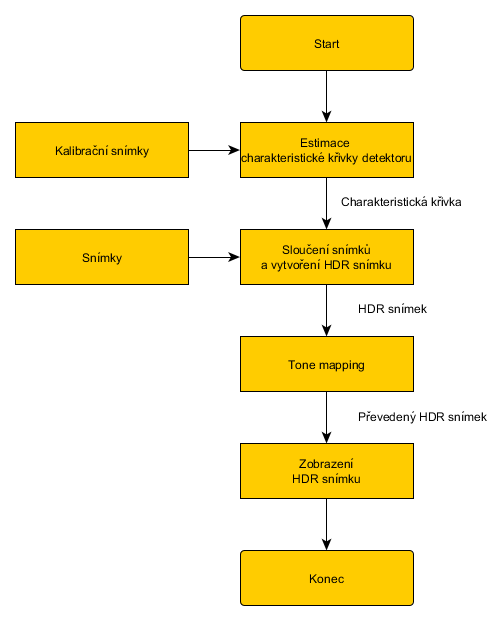
\includegraphics[width=12cm]{HDR-implementation}
\caption{Vývojový diagram implementace metody HDR.}
\label{fig:HDR-implementation}
\end{figure}

\subsubsection{Testovací data}
za účelem ověření správného fungování implementovaného Debevecova algoritmu byla nasnímána testovací a kalibrační data. Jako zdroj záření, stejně jako v předchozí kapitole, byla zvolena rentgenka Spellman XRB011 a detektor s CMOS snímači Shad-o-Box 1648 HS \cite{SB1548HS} od společnosti Teledyne Dalsa.

Pomocí této sestavy byly nasnímány dvě série snímků:
\begin{itemize}
\item Kalibrační snímky -- snímky sloužící pro estimaci odezvy detektoru. Tyto snímky byly nasnímány tak, aby na každém snímku byla alespoň jedna přeexponovaná, jedna podexponovaná oblast a alespoň jedna oblast, kde se mění intenzita se změnou expoziční doby $\Delta t$. Přeexponovaná oblast se v případě výše popsané sestavy nacházela ve všech místech přímého dopadu záření na detektor. Podexponovaná oblast byla vytvořena zastíněním části detektoru pomocí olověného plátu. Tímto způsobem byla nasnímána série snímků při \SI{60}{\kV} a \SI{250}{\micro\ampere} pro expoziční doby \SI{1000}{\ms}, \SI{500}{\ms}, \SI{250}{\ms}, \SI{125}{\ms} a \SI{60}{\ms}.
\item Testovací snímky -- snímky pro získání HDR snímku, které jsou nasnímány stejným způsobem, jako kalibrační snímky. Snímky by měly být nasnímány tak, aby snímek s nejnižší expozicí byl podexponován a snímek s nejvyšší expozicí naopak přeexponován. Tímto způsobem bylo opět nasnímáno 5 snímků při \SI{60}{\kV} a \SI{250}{\micro\ampere} pro expoziční doby \SI{1000}{\ms}, \SI{500}{\ms}, \SI{250}{\ms}, \SI{125}{\ms} a \SI{60}{\ms}.
\end{itemize}

\begin{figure}[htb]
\centering
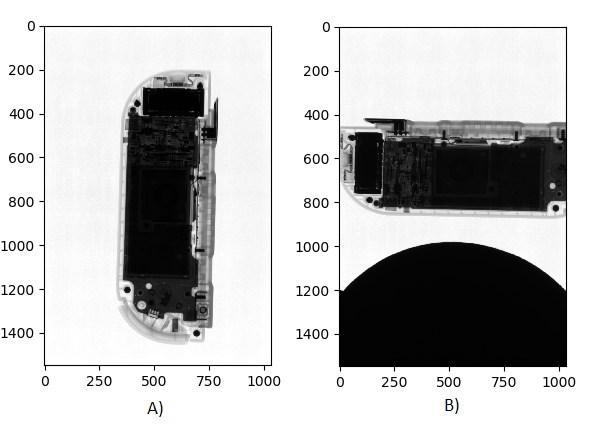
\includegraphics[width=\textwidth]{hdr-dataset-sample}
\caption{Testovací snímek (A) pro získání HDR snímku a kalibrační snímek (B) pro estimaci charakteristické křivky detektoru.}
\label{fig:hdr-dataset-sample}
\end{figure}

\paragraph{Předzpracování série testovacích snímků} bylo provedeno za účelem předpřipravení snímků pro aplikaci implementovaných metod. Kroky předzpracování je možné rozdělit do několika částí:
\begin{itemize}
\item Změna bytové hloubky snímků -- všechny snímky jsou nasnímány detektorem, který má 14 bitové AD převodníky. Z tohoto důvodu bylo nutné data  převést do 16 bitů, nebo 8 bitů, aby byl využit celý zobrazovací rozsah.
\item Předpřipravení snímků pro metody v OpenCV -- vzhledem k tomu, že OpenCV jako vstupní sérii snímků vyžaduje pole 3-kanálových snímků s bitovou hloubkou 8 bitů, bylo nutné každý snímek rozšířit o další dva kanály, do kterých byly nakopírovány hodnoty odpovídající původnímu kanálu, který reprezentoval odstíny šedi.
\end{itemize}

\subsubsection{Výsledky aplikace Debevecovy metody}
Na předzpracovaná data byl aplikován Debevecův algoritmus, který byl popsán výše. Nejdříve byla získána funkce odezvy detektoru $g$ a za pomocí této metody byl získán sloučením série testovacích dat HDR snímek. HDR snímek byl poté zobrazen pomocí čtyř tone mapping metod. Výsledný snímek lze vidět na obrázku \ref{fig:hdr-result}. Na výsledných snímcích je vidět krom zvýšeného dynamického rozsahu, také snížený šum díky skládání více snímků v jeden -- podobný princip jako v případě průměrování, kterému byla věnována předešlá kapitola. Zvýšený dynamický rozsah se projevil tak, že oproti testovacím snímkům v obrázcích \ref{fig:averaging-low-noise} a \ref{fig:hdr-dataset-sample} jsou na snímku zřetelná například tlačítka, které se nachází ve spodní části zařízení pod deskou plošného spoje. 

\begin{figure}[htb]
\centering
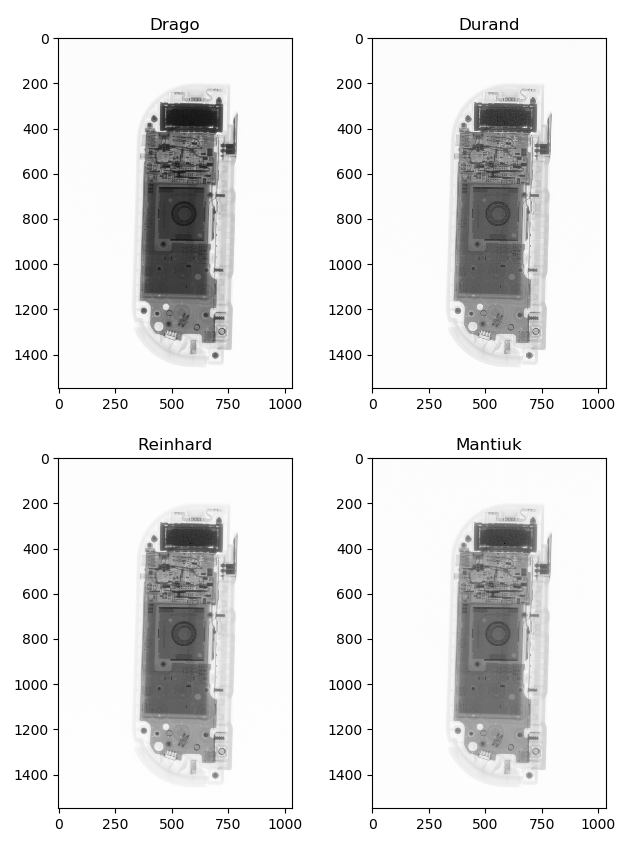
\includegraphics[width=\textwidth]{hdr-result}
\caption{Vygenerovaný HDR snímek zobrazený pomocí 4 tone mapping metod.}
\label{fig:hdr-result}
\end{figure}